\subsection{Problématique de la séparation d’étages dans les lanceurs expérimentaux}
\label{sec:problematique}

Un lanceur multi-étages est un véhicule spatial constitué de plusieurs segments successifs (étages) qui se détachent les uns
après les autres au cours du vol pour optimiser la masse propulsée et améliorer les performances. La séparation d’étages est la
transition mécanique et dynamique entre deux étages consécutifs, qui doit être réalisée de manière fiable et contrôlée pour
assurer la continuité de la mission en cours. Cette étape critique du vol implique des défis techniques majeurs, notamment en
termes de génération des forces nécessaires au détachement, de gestion des interactions aérodynamiques et de maintien de la
stabilité du véhicule.

\begin{quote}
    \textit{\og{}A separation mechanism that does not meet these requirements can produce attitude errors and tumble rates of the
    continuing body that are too large for its attitude-control system to accommodate, can damage its structure and critical
    equipment, and can cause failure or degradation of the mission.\fg{}}
    (cf. NASA Flight Separation Mechanisms\cite{NASA_Flight_Separation}).\\
\end{quote}

\begin{figure}[h!]
    \centering
    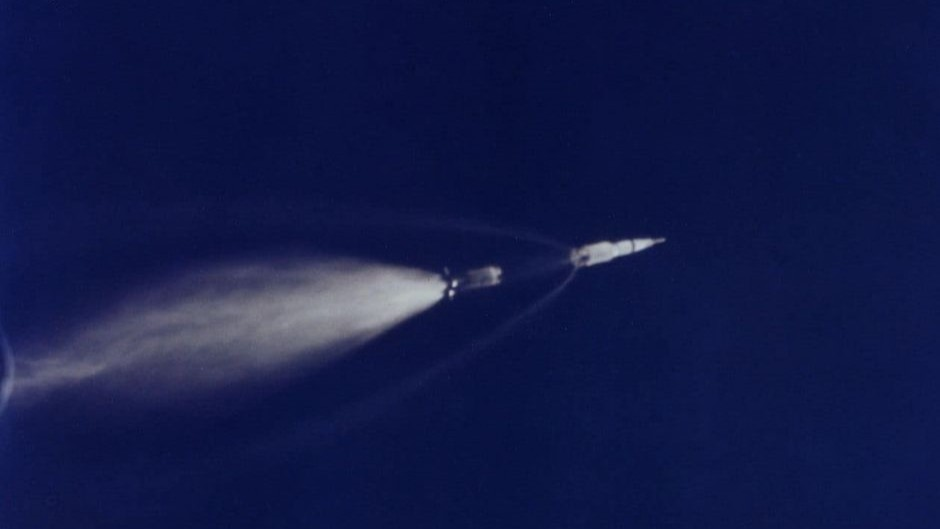
\includegraphics[width=0.9\textwidth]{figures/How-did-the-Saturn-V-stages-separate.jpg}
    \caption{Séparation des étages 1 et 2 du lanceur Saturn V~\cite{SaturnV_Separation}}
\end{figure}

Dans le domaine spatial industriel et commercial, les lanceurs (tels qu’Ariane 6, Falcon 9 ou Electron) exploitent des solutions
de séparation robustes et standardisées, souvent pyrotechniques, intégrées à des processus de qualification lourds. Ces systèmes
sont conçus pour une répétabilité élevée, des milliers d’heures de certification et des procédures de sûreté strictes. La taille,
la complexité et les ressources disponibles (budget, moyens d’essais, expertise) diffèrent radicalement de ceux des projets non
industriels.\\

À l’opposé se trouvent les lanceurs expérimentaux et les fusées sondes :
\begin{itemize}
    \item Un lanceur expérimental désigne généralement un véhicule développé dans un cadre académique ou associatif pour tester
    des concepts technologiques ou atteindre une performance définie dans des gammes de faible coût et faible volume.
    \item Une fusée sonde fait référence à un type de lanceur suborbital utilisé pour des missions scientifiques, des essais en
    atmosphère ou des validations de capteurs, souvent dans le contexte de programmes étudiants, de clubs aérospatiaux ou de
    projets de recherche gouvernementaux à budget limité.\\
\end{itemize}

Ces catégories se caractérisent par des échelles de taille et de masse très différentes des lanceurs commerciaux. Par exemple,
une fusée sonde ou expérimentale peut mesurer quelques mètres pour quelques dizaines de kilogrammes, alors qu’un lanceur orbital
pèse plusieurs centaines de tonnes et dépasse des dizaines de mètres de hauteur. Cette différence d’échelle se reflète directement
dans :
\begin{itemize}
    \item la simplicité de conception,
    \item les moyens de test disponibles,
    \item les contraintes réglementaires applicables,
    \item les budgets alloués,
    \item et les exigences de fiabilité opérationnelle.\\
\end{itemize}

\begin{figure}[h!]
    \centering
    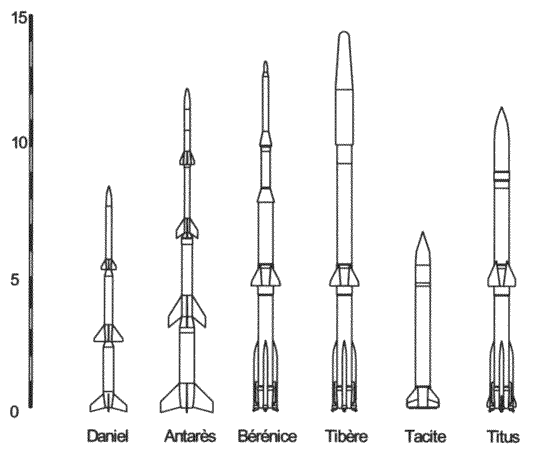
\includegraphics[width=0.6\textwidth]{figures/onera.png}
    \caption{Famille de lanceurs expérimentaux et de fusées sondes développés par l'ONERA~\cite{Onera_Family}}
\end{figure}

Dans ce contexte, la séparation d’étages représente un défi particulier. Les solutions héritées du domaine industriel
(pyrotechnique ou très mécanisées) ne sont pas toujours adaptées à des véhicules de petite échelle, car elles peuvent être
surdimensionnées en termes de charge ou de complexité, nécessiter des procédures d’essai lourdes difficiles à exécuter avec des
moyens limités ou imposer des coûts prohibitif pour des projets à budget restreint.\\

La problématique étudiée dans ce rapport vise donc à comprendre et analyser les solutions possibles de séparation adaptées à ces
contraintes particulières : simplicité, intégration minimale, facilité de test, et compatibilité avec des processus de
développement itératifs. Cette réflexion justifie une investigation des principes existants, suivie d’une exploration dédiée de
solutions compatibles avec les objectifs et la philosophie des lanceurs expérimentaux et des fusées sondes.
